\apendice{Documentación técnica de programación}

\section{Introducción}

\section{Estructura de directorios}
Hay que conocer las diferentes partes del proyecto y tener en cuenta que son completamente diferentes aunque en este proyecto se han integrado para poder hacer uso del sistema domótico. Podemos ver una primera distribución general en la imagen~\ref{Img:PartesProyecto}. En ella podemos diferenciar tres partes principales:

Tuve un problema generalizado en el código puesto que obtenía las rutas a los archivos de forma unitaria desde el archivo en ejecución. Este es el código utilizado para obtener la ruta en Python:
\begin{lstlisting}[language=json,firstnumber=0]
{
    #!/usr/bin/env python3
    #Calculamos ruta
    ruta=os.getcwd().split('/')
}
\end{lstlisting}

Éste es el código utilizado para obtener la ruta en Bash:
\begin{lstlisting}[language=json,firstnumber=0]
{
    #!/bin/bash
    path=$(pwd)
}
\end{lstlisting}

\begin{itemize}
    \item La parte de toma de datos.
    \item La parte de mensajería.
    \item La parte física de nuestra instalación domótica, incluyendo la Raspberrry Pi.
\end{itemize}

\begin{figure}
    \centering
    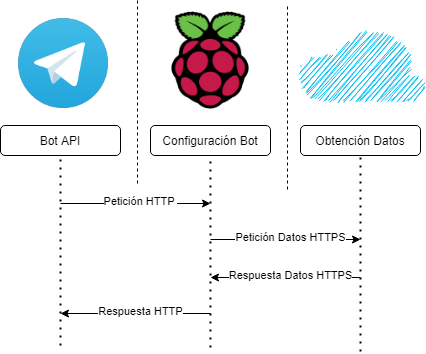
\includegraphics[width=0.7\textwidth]{img/PartesProyecto.png}
    \caption{Partes del proyecto. } \label{Img:PartesProyecto}
\end{figure}

Por ello, el código se ha estructurado en tres partes:
\begin{itemize}
    \item La carpeta \textbf{auto}, que permite obtener la información de las APIs seleccionadas de Internet.
    \item La carpeta \textbf{bot}, donde almacenamos la configuración de nuestro bot.
    \item La carpeta \textbf{control}, donde almacenamos los scripts de control de la instalación domótica.
\end{itemize}

En todas ellas, los scripts, tanto de Bash como de Python llevan la cabecera específica para el tipo de código contenido en el archivo:

\begin{lstlisting}[language=json,firstnumber=0]
{
    #!/usr/bin/env python3
}
\end{lstlisting}

Éste es el código utilizado para obtener la ruta en Bash:
\begin{lstlisting}[language=json,firstnumber=0]
{
    #!/bin/bash
}
\end{lstlisting}


Para los archivos Python, la sentencia <<#!/usr/bin/env python3>> y para los archivos Bash, la sentencia <<#!/bin/bash>>. He introducido esta cabecera porque he tenido problemas al lanzar las instrucciones desde otro script.

\subsection{Carpeta auto}
Al comienzo del proyecto esperé encontrar alguna web desde la que poder recoger la información haciendo webscraping pero tras valorarlo detenidamente en las tutorías prefería a buscar una API (ver concepto~\ref{concepto:API}). Uno de los motivos es que una web es más susceptible de sufrir cambios que una API que se ha predispuesto para una función.
Finalmente, dispuse el proyecto para poder funcionar con dos APIs públicas y gratuitas para dotar a nuestro sistema domótico de autonomía.
Las siguientes fases de la parte de toma de datos, se albergan en la carpeta auto ya que es un proceso automatizado que permite al sistema obtener los datos de forma desatendida y continua.
El proceso de automatización comprende varias fases:
\begin{enumerate}
    \item La fase de recopilación de datos.
    \item La fase de lectura local de parámetros.
    \item El cocinado de los datos.
    \item El grabado de datos en el sistema local.
\end{enumerate}
La fase de recopilación de datos llama a la API de geolocalización y nos devuelve, entre otros, los parámetros de nuestra ubicación en formato de latitud y longitud. Posteriormente, estos datos de ubicación son necesarios para incorporarlos en la consulta de la siguiente API~\ref{4:API_Tiempo} y obtener la información de la salida y puesta del sol así como la información de las temperaturas del día siguiente en dicha ubicación. Con esta recopilación de datos tenemos la base para poder determinar el comportamiento autónomo que necesitamos por lo que almacenaremos esta información en un archivo de datos.

El siguiente paso es leer las preferencias del usuario, que se almacenan en el archivo de condicionantes. Y, una vez tengamos estos datos, podemos pasar a generar el Cron para controlar de forma automática toda la instalación.

Estas fases se han confeccionado al final del proyecto puesto que al principio se desarrolló de forma unitaria pero surgió el problema de que, cada vez que queríamos hacer una modificación en el sistema domótico de cualquier índole, teníamos que hacer una petición nueva a las APIs y generar de nuevo un archivo Cron con los parámetros del usuario <<al vuelo>> para conseguir regenerar la automatización con los parámetros nuevos. Este sistema funcionaba correctamente pero era poco eficiente puesto que que se multiplican las operaciones en función de las veces que se quiera modificar algún parámetro.
Únicamente he permitido realizar dos salidas "al vuelo" tras obtener los datos, estos son: el grabado de los datos recién obtenidos y la gráfica de las temperaturas conforme a dichos datos.

He tenido algunos problemas al realizar varias peticiones a las APIS ya que, por falta de permisos, no podía sobreescribir los archivos ni las imágenes. Para subsanarlo, incluí una restricción para modificar los permisos de los archivos de forma que únicamente pueden acceder el propietario y el grupo.

\subsection{Carpeta control}
La carpeta control alberga aquellos scripts bash que controlan los elementos domóticos. Este punto únicamente me dio problemas a la hora de implantarlo desde el bot, que se subsanó con la librería os.

\subsection{Carpeta bot}
La carpeta bot contiene varios archivos, desde el archivo de control del bot hasta otros que contienen la mayoría de funcionalidades de éste. En primera instancia, se dispuso todo el código dentro del archivo de control del bot, pero por legibilidad y facilidad de mantenimiento se extrajeron las funciones.
En este punto, lo que más problemas me ha dado han sido los teclados. Como comportamiento de los teclados es diferente entre ellos tendría que dividir las opciones del bot entre dos tipos de teclados diferentes. Finalmente, opté por no incluir estos teclados ya que no incluye funcionalidad alguna y disminuirían la legibilidad y facilidad de uso del bot. Además, para aumentar la usabilidad del bot, se ha dispuesto un menú que podemos ver al introducir el carácter "/" además de la posibilidad de utilizar la primera letra del comando siempre que no tengamos que acompañarlo de parámetros.

\subsection{Configuración del bot como servicio}
El bot se puede lanzar como si fuera un script más pero en este caso es necesario incorporarlo como servicio. Esta decisión tiene beneficios como la posibilidad de que se inicie con el sistema o que podamos lanzarlo o pararlo desde cualquier ubicación del SO sin tener que recordar la ubicación con la sentencia al efecto de <<\textbf{sudo service bot start/stop}>>. Pero, una vez que el demonio está corriendo, tenemos que tener en cuenta de que ya está levantada la instancia del bot, por lo que tendremos que detenerla a la hora de hacer algún tipo de modificación así como recordar que debemos levantarlo una vez terminemos.



\section{Manual del programador}

\section{Compilación, instalación y ejecución del proyecto}

\section{Pruebas del sistema}


